\chapter{Experiments}\label{experiments}
This chapter aims to test methods described in earlier chapters. We describe
setup and context for the experiments as well as what data was used.

The experiments described in this chapter are the following. Dictionary
compilation, \ref{experiments:dictionaries}. The word count classification, bag
of words method, \ref{experiments:word_count_classification}. Threshold
variation in section \ref{experiments:threshold}. Kernel choice for the SVM
classifier is described in section \ref{experiments:svm_kernel}. With the
testing of classifiers coming next, \ref{experiments:calssifiers}. And the trend
aggregation comes last in section \ref{experiments:trend}.

\section{Dictionary compilation}\label{experiments:dictionaries}
Section \ref{data:dictionaries} describes dictionaries and what they are used
for. This section describes how the dictionaries are tested. 
The dictionaries are compiled from manually labeled tweets.

As a step in the sentiment classification dictionaries was created for the
word count classification \ref{sentiment:word_count_classification}.
To find out which dictionaries performed well or not we tested the dictionaries
with two data sets, the kiro dataset and the obama dataset. 

This experiment enlightens part of research question 1,
\ref{introduction:rq1}, how we can find the sentiment of a tweet.

\paragraph{Dictionary quality}
\hspace{0pt}\\
To test the dictionary quality the word count classification
\ref{experiments:word_count_classification} does it for us. All the
dictionaries are tested with the two datasets and we can compare the results. 
How the dictionaries are compiled are described in
\ref{data:compiled_dictionaries} and \ref{code:dictionary_compilation}.

\paragraph{Removal of duplicate words}
\hspace{0pt}\\
When creating the different dictionaries we remove duplicates from the positive
and negative dictionary set. Words that are present in both the positive and
negative dictionary is removed. By doing this we remove words that has no
significance in the classification. But we also risk removing words with
significance.

The code is described in appendix \ref{code:remove_duplicate_words} on page
\pageref{code:remove_duplicate_words}.

\paragraph{Results}
\hspace{0pt}\\
Results from the testing of dictionaries are closely linked to the word count
classification in \ref{experiments:word_count_classification} and described in
table \ref{tbl:sentiment_word_count_results} on page
\pageref{tbl:sentiment_word_count_results}.
%

\section{Word Count Classification}\label{experiments:word_count_classification}
Inspiration from section \ref{previous_work:sentiment}, with knowledge of tweets
and dictionaries in section \ref{data:tweets}, builds this experiment. The
background for the experiment and how it's purpose is described in section
\ref{sentiment:classification}. 

This experiment used the technique described in section
\ref{sentiment:word_count_classification}, the word count method of classifying
a tweets sentiment.  

This experiment tries to expand on the matter of how to determine the sentiment
of a tweet, \ref{introduction:rq1}. And how Twitter can be used, indirectly, to
aggregate a trend, \ref{introduction:rq2}.
The method looks at at the amount of positive and negative words and use
that to decide the sentiment.

For all the dictionaries and datasets, the classification process is run. This
gives the accuracy for all dictionaries and the two datasets. This in turn
describes the efficiency of the word count classification.

The code for calculating the sentiment is as follows. It is also described in
appendix \ref{code:word_count_classification}, on page
\pageref{code:word_count_classification}.
\begin{python}
positivity = positive_words_count / total_number_words
negativity = negative_words_count / total_number_words

polarity = positivity - negativity

if polarity > 0:
    tweet is positive
else:
    tweet is negative
\end{python}

The results of the classification can be found in section
\ref{results:word_count_classification} on page
\pageref{results:word_count_classification}.
%

\section{Threshold Variation}\label{experiments:threshold}
In section \ref{sentiment:threshold} the description an purpose of the
threshold variation is described. The threshold aims to find out how positive a
tweet has to be before it is actually positive. Or rather how many more
positive words than negative words do we need to call the tweet positive. 

By varying the threshold we hoped to find an optimal point of which we could
separate tweets based on polarity. From the following
graphs, figure \ref{fig:threshold_graphs}, we can see no clear distinction of
one value being better than the other ones.

In essence what is done is that the word count classification is run multiple
times where the threshold value is changed between -0.9 and 0.9. This give a
distribution of results which is plotted in graph
\ref{fig:average_threshold_accuracy} on page
\pageref{fig:average_threshold_accuracy}.
The results will give an indication of what threshold is best for word
word counting. 

The results of the threshold variation is described in section
\ref{results:threshold}, on page \pageref{results:threshold}. And in table
\ref{tbl:average_threshold_accuracy} on page
\pageref{tbl:average_threshold_accuracy}.
%


\section{Choice of SVM Kernel}\label{experiments:svm_kernel}
In extension of \ref{sentiment:svm_classification} all the SVM kernels were tested. 
While testing which kernel was best we used the kiro dataset for training, and
the kiro monogram dictionary for feature extraction.

Using the self compile monogram dictionaries and all the different SVM kernels
we get these results:

\begin{table}
\centering
\label{tbl:svm_classifier_kernel_test}
\caption{SVM kernel test results table}
\begin{tabular}{ l r r c }
Kernel & Failed & Correct & Accuracy \\
\hline
LinearSVC & 7 & 990 & 0.9930 \\
NuSVC & 29 & 968 & 0.9709 \\
NuSVR & 422 & 575 & 0.5767 \\
OneClassSVM & 575 & 422 & 0.4233 \\
SVC & 422 & 575 & 0.5767 \\
SVR & 422 & 575 & 0.5767 \\
\end{tabular}
\end{table}
%

\section{With Classifiers}\label{experiments:calssifiers}
For the classifiers the two datasets was tested with the two classifiers.
This was done to find the best classifier and compare the results
with the word count classification. By confirming that classifiers are better
than word counting we can eliminate a factor in the classification
uncertainties. 

The description of the comparison on a conceptual level is described in section
\ref{sentiment:comparison_results}. Also of interest there is the element of
the dictionaries in section \ref{data:dictionaries}. While we have taken
inspiration and ideas for the experiment from section
\ref{previous_work:sentiment}.

For the research questions to be enlightened further here is the trend
aggregation in section \ref{introduction:rq1} and the sentiment determination
in section \ref{introduction:rq2}.

\paragraph{SVM}\label{experiments:svm_classification}
\hspace{0pt}\\
Results from testing SVM with different dictionaries are described in table
\ref{tbl:svm_classifier_results} on page
\pageref{tbl:svm_classifier_results}.

\begin{table}
\centering
\label{tbl:svm_classifier_results}
\caption{SVM classifier results table}
\begin{tabular}{ l l r r c }
Dataset & Type & Failed & Correct & Accuracy \\
\hline
Kiro & Monogram & 7 & 990 & 0.9930 \\
Kiro & Bigram & 422 & 575 & 0.5767 \\
Obama & Monogram & 35 & 1330 & 0.9744 \\
Obama & Bigram & 507 & 858 & 0.6286 \\
\end{tabular}
\end{table}

\paragraph{Naive Bayes}\label{experiments:naive_bayes_classification}
\hspace{0pt}\\
Results from testing Naive Bayes with different dictionaries are described in
table \ref{tbl:naive_bayes_classification_results} on page
\pageref{tbl:naive_bayes_classification_results}.

\begin{table}
\centering
\label{tbl:naive_bayes_classification_results}
\caption{Naive Bayes classifier results table}
\begin{tabular}{ l l r r c }
Dataset & Type & Failed & Correct & Accuracy \\ 
\hline 
Kiro & Monogram & 29 & 968 & 0.9709 \\
Kiro & Bigram & 29 & 968 & 0.9709 \\
Obama & Monogram & 59 & 1306 & 0.9568 \\
Obama & Bigram & 59 & 1306 & 0.9568 \\
\end{tabular}
\end{table}
%

\section{Trend aggregation}\label{experiments:trend}
Before executing this experiment section \ref{trend:compared} describes the
conceptual parts of the trend comparison. This is the basis for the results of
this experiment. 

This experiment aims to test the relevance of positive and negative tweets in
correlation with change in finance. There are two parts of this experiment. The
finance part, and the twitter part. Can twitter be used to create a trend,
\ref{introduction:rq2}. And how can we compare this to a finance trend,
\ref{introduction:rq3}.

In the execution of the experiment the methods described in chapter \ref{trend}
has been used. More specifically the trend aggregation under trends on twitter,
\ref{trend:trends_on_twitter}. And the finance trend aggregation,
\ref{trend:trends_in_finance}.

The tweet data used is described in section \ref{data:trend_data}, on page
\pageref{data:trend_data}. And the finance data is described in section
\ref{data:finance}, page \pageref{data:finance}.

The results of the experiment are discussed in section \ref{results:trend}.

\paragraph{Finance plot}
The plotting of the graph is described in better detail in appendix
\ref{code:trend_aggregation}, page \pageref{code:trend_aggregation}.

Plotting the finance trend we got figure \ref{fig:trend_finance_plot}, page
\pageref{fig:trend_finance_plot}.
\begin{figure}[htb]
    \centering
    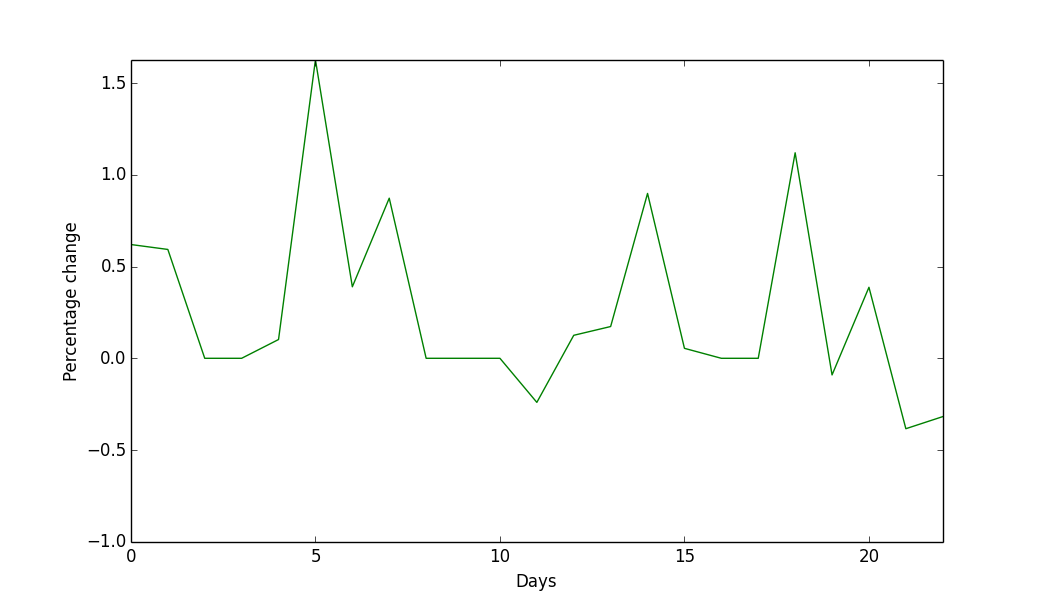
\includegraphics[width=\textwidth]{finance_trend_plot.png}
    \label{fig:trend_finance_plot}
    \caption{Finance trend plot}
This is the plot for OSEBX. The plot show the moving average in the middle and
the Average directional graph at the bottom.
\end{figure}


\paragraph{Twitter plot}
Code for plotting the trend graph is described in appendix
\ref{code:trend_aggregation}, page \pageref{code:trend_aggregation}.

Plotting the moving average for the Twitter trend we get figure:
\ref{fig:trend_tweet_plot}, on page
\pageref{fig:trend_tweet_plot}.

\begin{figure}[htb]
    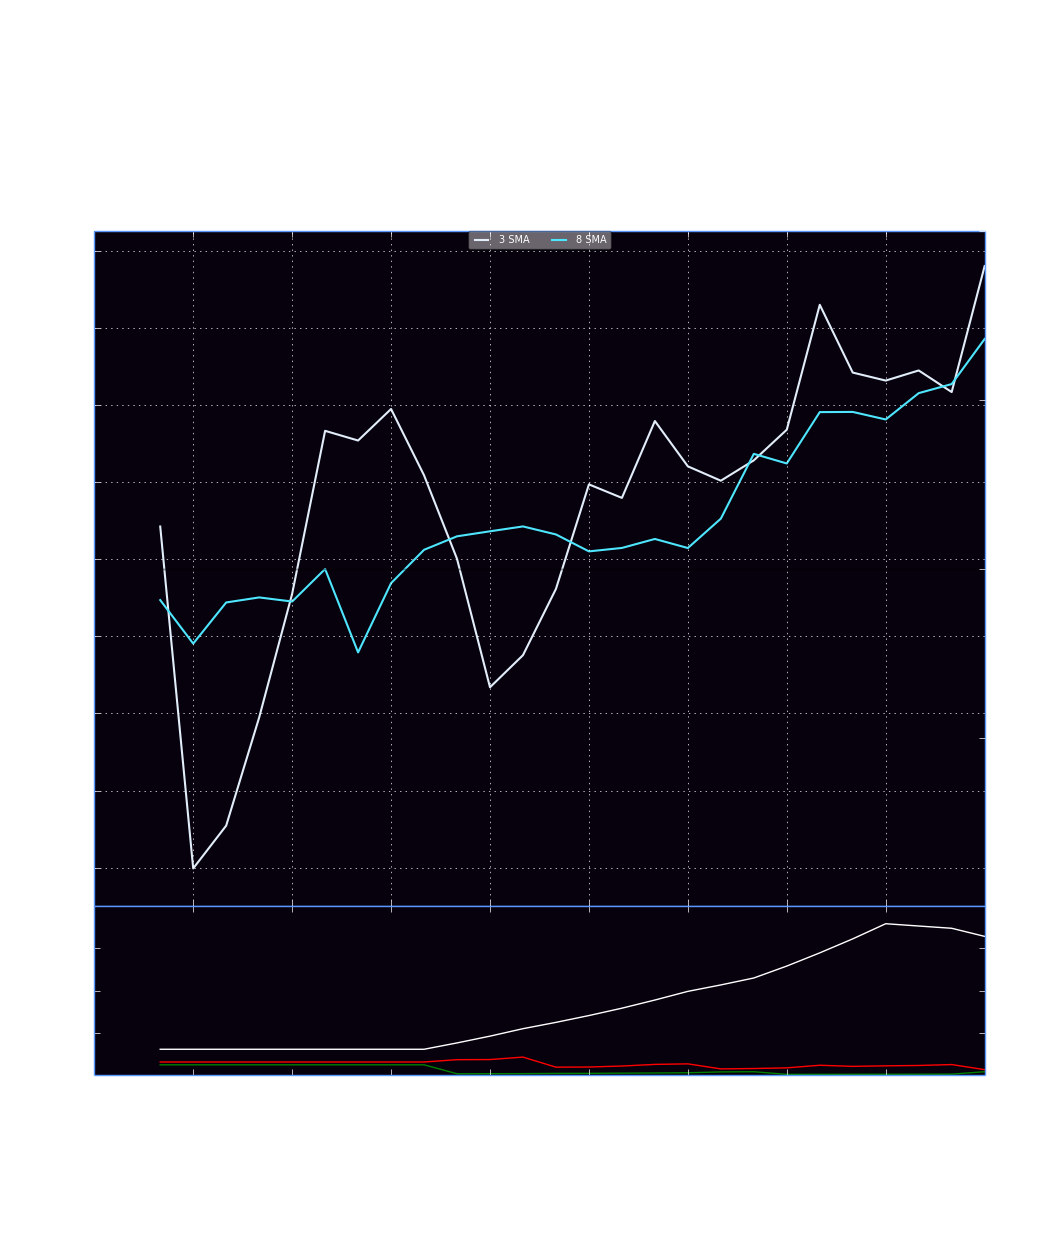
\includegraphics[width=\textwidth]{tweet_trend_plot.png}
    \label{fig:trend_tweet_plot}
    \caption{Tweet trend plot}
This is the Twitter trend plot. The plot show the moving average in the middle
and the Average directional graph at the bottom.
\end{figure}
%

